\documentclass[../../main.tex]{subfiles}
\begin{document}

{\bf [解答]} ただし$0\le\theta<2\pi$とする．
$P$が$xy$平面上の円$x^2+y^2=16a^2$上を動くよう，$N(a/2,0,\sqrt{3}a/2)$とする．
すると$P(4ac,4as)$と置ける．$N$での$S$の接平面$T$は
\begin{align}
  T:\dfrac{a}{2}x+\dfrac{\sqrt{3}a}{2}z=a^2
\end{align}
であり，これと$xy$平面との交線は$x=2a$となり，下図のようになる．

\begin{figure}[htb]
  \centering
  % 左パネル: 3次元空間における球面 S, 点 N, 接平面と xy 平面の交線
  \begin{subcaptionblock}{0.48\textwidth}
    \centering
    \begin{tikzpicture}[scale=1.1, >=stealth, every node/.style={font=\small}]
      \coordinate (O) at (0, 0);

      % 座標軸
      \draw[->, thick, gray!80!black] (O) -- (2.8, 0) node[right] {$x$};
      \draw[->, thick, gray!80!black] (O) -- (0, 2.5) node[above] {$z$};
      \draw[->, thick, gray!80!black] (O) -- (-1.3, -1.3) node[below left] {$y$};
      \node[below left=1pt, font=\footnotesize] at (O) {$O$};

      % 球面 S の輪郭 (半径 a = 1.0)
      \draw[line width=1.1pt, gray!85!black] (O) circle (1.0);
      % 赤道円 (奥: 破線, 手前: 実線)
      \draw[densely dotted, thick, gray!70!black] (1.0, 0) arc[start angle=0, end angle=180, x radius=1.0, y radius=0.32];
      \draw[thick, gray!70!black] (-1.0, 0) arc[start angle=180, end angle=360, x radius=1.0, y radius=0.32];

      % 点 N (a/2, 0, sqrt(3)/2 a) = (0.5, 0, 0.866)
      \coordinate (N) at (0.5, 0.866);
      \draw[thick, dashed, gray!70!black] (O) -- (N);
      \node[circle, fill=blue!85!black, inner sep=1.3pt] at (N) {};
      \node[above right=1pt, font=\footnotesize, blue!85!black] at (N) {$N$};

      % 円軌道 (半径 4a = 2.2 に縮尺)
      \draw[thick, dashed, gray!60!black] (2.2, 0) arc[start angle=0, end angle=360, x radius=2.2, y radius=0.75];
      \coordinate (P) at (1.8, -0.45);
      \node[circle, fill=red!85!black, inner sep=1.3pt] at (P) {};
      \node[below right=1pt, font=\footnotesize, red!85!black] at (P) {$P$};

      % 視線 NP
      \draw[line width=1.0pt, red!80!black] (N) -- (P);

      % 接平面の交線 x = 2a (z=0 上の直線, y 軸に平行)
      \coordinate (L1) at ($(1.8, 0) + (-0.7, -0.7)$);
      \coordinate (L2) at ($(1.8, 0) + (0.7, 0.7)$);
      \draw[line width=1.2pt, teal!85!black] (L1) -- (L2) node[above right=1pt, font=\footnotesize] {$x=2a$};
      \node[below=3pt, font=\footnotesize] at (2.0, -0.1) {$2a$};
    \end{tikzpicture}
    \caption{空間における球面 $S$ と点 $N, P$}
  \end{subcaptionblock}
  \hfill
  % 右パネル: xy 平面における円軌道と可視領域 x >= 2a
  \begin{subcaptionblock}{0.48\textwidth}
    \centering
    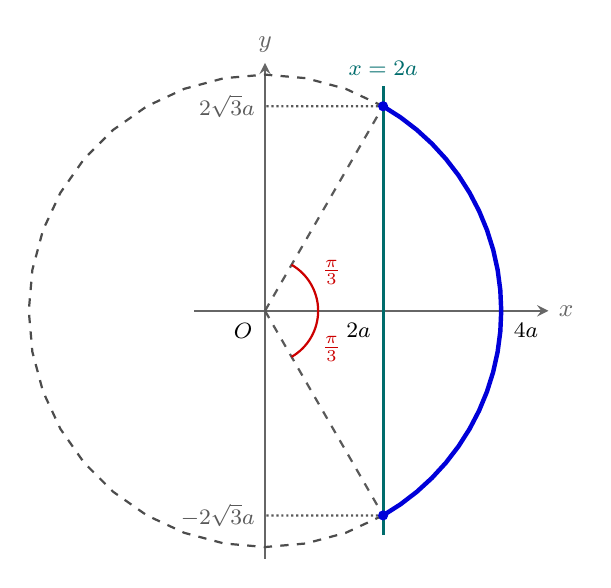
\begin{tikzpicture}[scale=0.75, >=stealth, every node/.style={font=\small}]
      \coordinate (O) at (0, 0);

      % 座標軸
      \draw[->, thick, gray!80!black] (-1.2, 0) -- (4.8, 0) node[right] {$x$};
      \draw[->, thick, gray!80!black] (0, -4.2) -- (0, 4.2) node[above] {$y$};
      \node[below left=1pt, font=\footnotesize] at (O) {$O$};

      % 可視領域の円弧 (4a = 4cm, theta = -60 to 60)
      \draw[line width=1.6pt, blue!85!black, domain=-60:60]
      plot ({4*cos(\x)}, {4*sin(\x)});

      % 見えない部分の円軌道 (破線)
      \draw[thick, dashed, gray!60!black, domain=60:300]
      plot ({4*cos(\x)}, {4*sin(\x)});

      % 直線 x = 2a
      \draw[line width=1.1pt, teal!85!black] (2, -3.8) -- (2, 3.8)
      node[above, font=\footnotesize] {$x=2a$};
      \node[below left=1pt, font=\footnotesize] at (2, 0) {$2a$};
      \node[below right=1pt, font=\footnotesize] at (4, 0) {$4a$};

      % 半径線と角度
      \coordinate (Q1) at ({4*cos(60)}, {4*sin(60)});
      \coordinate (Q2) at ({4*cos(-60)}, {4*sin(-60)});
      \draw[dashed, thick, gray!70!black] (O) -- (Q1);
      \draw[dashed, thick, gray!70!black] (O) -- (Q2);

      \draw[thick, red!80!black] (0.9, 0) arc[start angle=0, end angle=60, radius=0.9];
      \node[text=red!80!black, fill=white, inner sep=0.8pt, font=\footnotesize] at (30:1.3) {$\frac{\pi}{3}$};
      \draw[thick, red!80!black] (0.9, 0) arc[start angle=0, end angle=-60, radius=0.9];
      \node[text=red!80!black, fill=white, inner sep=0.8pt, font=\footnotesize] at (-30:1.3) {$\frac{\pi}{3}$};

      % 交点と座標
      \draw[densely dotted, thick, gray!70!black] (Q1) -- (0, {4*sin(60)}) node[left, font=\footnotesize] {$2\sqrt{3}a$};
      \draw[densely dotted, thick, gray!70!black] (Q2) -- (0, {4*sin(-60)}) node[left, font=\footnotesize] {$-2\sqrt{3}a$};

      \node[circle, fill=blue!85!black, inner sep=1.3pt] at (Q1) {};
      \node[circle, fill=blue!85!black, inner sep=1.3pt] at (Q2) {};
    \end{tikzpicture}
    \caption{$xy$ 平面における可視領域（太線部）}
  \end{subcaptionblock}
  \caption{球面 $S$ による点 $P$ の観測条件}
  \label{fig:sphere_visibility}
\end{figure}

$P$が見えるのは$2a\le x$の領域である．これは$-\pi/3\le\theta\le\pi/3$の領域であるから，見え続ける時間$t$として
\begin{align}
  \dfrac{\pi}{12}t=\dfrac{2\pi}{3} \Longleftrightarrow t=8
\end{align}
である．$\cdots$(答)

次に，$f(\theta)=|NP|^2$とおくと，
\begin{align}
  f(\theta)&=\left(4ac-\dfrac{a}{2}\right)^2+(4as)^2+\left(\dfrac{\sqrt{3}a}{2}\right)^2 \\
  &=a^2\left[16c^2-4c+\dfrac{1}{4}+16s^2+\dfrac{3}{4}\right] \\
  &=a^2\left[-4c+17\right]
\end{align}
である．この$-\pi/3\le\theta\le\pi/3$での最大小を求めればよく，$|NP|\ge0$ゆえ，
\begin{align}
  &
  \begin{cases}
    \max f(\theta)=f\left(\pm\dfrac{\pi}{3}\right)=15a^2 \\
    \min f(\theta)=f(0)=13a^2
  \end{cases} \\
  \therefore \
  &
  \begin{cases}
    \max |NP|=\sqrt{15}a \\
    \min |NP|=\sqrt{13}a
  \end{cases}
\end{align}
である．$\cdots$(答)

\newpage
\end{document}
